\section{Обзор предметной области} 
\label{review}

В данной главе представлен обзор предметной области, связанной с проблемой инвариантности к сдвигам в сверточных нейронных сетях. Рассматриваются ключевые аспекты проблемы, существующие методы оценки и улучшения инвариантности, а также особенности проявления проблемы в различных типах архитектур. Особое внимание уделено современным подходам к антиалиасингу в нейронных сетях и специфике проблемы в контексте детекторов объектов.

\subsection{Сверточные нейронные сети}
\label{review:cnn}

Сверточные нейронные сети (Convolutional Neural Networks, CNN) представляют собой класс глубоких нейронных сетей, специально разработанных для эффективной обработки данных с сеточной структурой, таких как изображения \cite{lecun1998gradient}. В отличие от традиционных полносвязных нейронных сетей, CNN используют операцию свёртки, что значительно уменьшает количество параметров и вычислительную сложность, сохраняя при этом способность к обучению сложным пространственным паттернам.

\subsubsection{Операция свёртки}
\label{review:cnn:convolution}

Ключевым элементом CNN является операция свёртки, которая заключается в применении фильтра (или ядра) к входным данным. Математически дискретная двумерная свёртка может быть выражена следующим образом:

\begin{equation}
(I * K)(i, j) = \sum_{m}\sum_{n} I(i+m, j+n) \cdot K(m, n)
\end{equation}

где $I$ — входное изображение, $K$ — ядро свёртки, а $*$ — операция свёртки. В контексте глубоких нейронных сетей применяется кросс-корреляция:

\begin{equation}
(I * K)(i, j) = \sum_{m}\sum_{n} I(i-m, j-n) \cdot K(m, n)
\end{equation}

\begin{figure}[h]
\centering
% Здесь будет рисунок, иллюстрирующий операцию свёртки в CNN
\caption{Иллюстрация операции свёртки в CNN}
\label{fig:convolution}
\end{figure}

Ядро свёртки «скользит» по входному изображению, вычисляя взвешенную сумму значений пикселей под ним для каждой позиции. Это позволяет нейронной сети обнаруживать различные признаки изображения, такие как края, текстуры и более сложные паттерны на более высоких уровнях абстракции.

\subsubsection{Архитектура сверточных нейронных сетей}
\label{review:cnn:architecture}

Типичная архитектура CNN состоит из нескольких ключевых компонентов:

\begin{itemize}
    \item \textbf{Сверточные слои} — основные строительные блоки, применяющие операцию свёртки для извлечения признаков изображения.
    \item \textbf{Слои субдискретизации (пулинга)} — уменьшают пространственную размерность данных, сохраняя наиболее важную информацию. Наиболее распространены max-pooling (выбор максимального значения в окне) и average-pooling (усреднение значений в окне).
    \item \textbf{Слои активации} — применяют нелинейные функции к выходам сверточных слоев, обычно ReLU (Rectified Linear Unit), что позволяет сети моделировать сложные нелинейные зависимости.
    \item \textbf{Полносвязные слои} — обычно располагаются в конце сети и используются для классификации на основе извлеченных признаков.
    \item \textbf{Слои нормализации} — стабилизируют и ускоряют процесс обучения (например, Batch Normalization).
\end{itemize}

\begin{figure}[h]
\centering
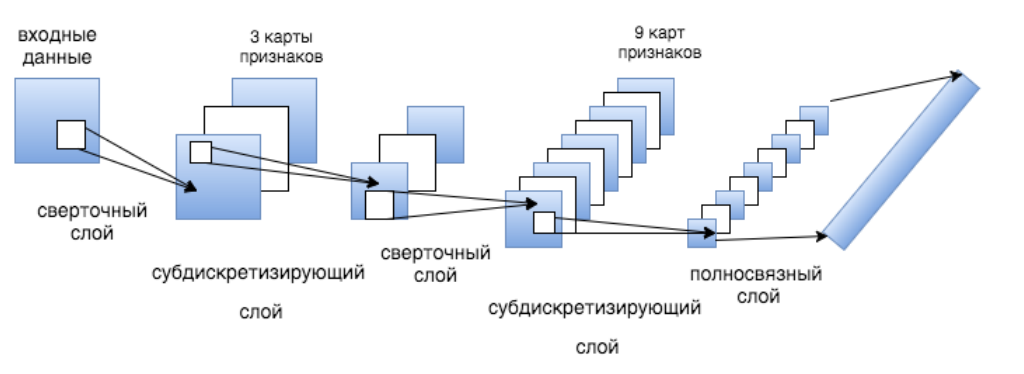
\includegraphics[width=0.95\textwidth]{figures/typical_cnn.png}
\caption{Типичная архитектура сверточной нейронной сети}
\label{fig:cnn_architecture}
\end{figure}

Данная архитектура обеспечивает два ключевых свойства CNN: разделение параметров (параметры ядра используются повторно для всего изображения) и локальные рецептивные поля (каждый нейрон обрабатывает только небольшую область входных данных).

\subsubsection{Эквивариантность и инвариантность к преобразованиям}
\label{review:cnn:invariance_concepts}

В контексте нейронных сетей важно различать два ключевых понятия:

\begin{itemize}
    \item \textbf{Эквивариантность} — свойство функции, при котором преобразование входных данных приводит к соответствующему преобразованию выходных данных. Формально функция $f$ эквивариантна к преобразованию $T$, если $f(T(x)) = T(f(x))$.
    \item \textbf{Инвариантность} — свойство функции, при котором преобразование входных данных не влияет на выходные данные. Формально функция $f$ инвариантна к преобразованию $T$, если $f(T(x)) = f(x)$.
\end{itemize}

Операция свёртки математически эквивариантна к сдвигам: если входное изображение сдвигается, то соответствующим образом сдвигаются и карты признаков. Однако полная сеть CNN должна обладать инвариантностью к сдвигам на уровне итоговой классификации — позиция объекта на изображении не должна влиять на результат распознавания.

Теоретически, сочетание эквивариантности сверточных слоев и операций пулинга должно обеспечивать определенную степень инвариантности к пространственным трансформациям, включая сдвиги. Однако, как будет показано далее, современные CNN на практике демонстрируют ограниченную инвариантность к сдвигам.

\subsection{Инвариантность к сдвигу в CNN-классификаторах}
\label{review:invariance}

Сверточные нейронные сети (CNN) теоретически должны обладать определенной степенью инвариантности к позиционным сдвигам входных данных благодаря механизму разделения весов и локальным рецептивным полям \cite{Zhang2019blurpool}. Однако, как показывают исследования последних лет, современные CNN демонстрируют ограниченную инвариантность к сдвигам, что противоречит интуитивным ожиданиям.

Исторически, LeCun et al. \cite{lecun1998gradient} первыми формально описали свойство эквивариантности сверточных сетей к сдвигам, выделив ключевые свойства CNN — локальность связей, разделение весов и пространственный пулинг. Теоретически, операция свёртки обладает эквивариантностью к сдвигам: если входное изображение сдвигается, то соответствующим образом сдвигаются и карты признаков.

Несмотря на теоретические предпосылки, эмпирические исследования выявили существенные ограничения в инвариантности современных CNN к сдвигам. Engstrom et al. \cite{engstrom2019exploring} продемонстрировали, что даже небольшие сдвиги входных изображений могут значительно снизить точность классификации современных архитектур, включая ResNet.

Zhang \cite{Zhang2019blurpool} в своем фундаментальном исследовании идентифицировал операции даунсэмплинга (max-pooling и свертку с шагом больше 1) как основной источник нарушения инвариантности к сдвигам. Автор показал, что субпиксельные сдвиги входных изображений приводят к значительным изменениям в активациях нейронов и нестабильности предсказаний модели.

Azulay and Weiss \cite{azulay2019deep} продемонстрировали, что проблема инвариантности может быть систематически исследована через призму классической теории обработки сигналов. Отсутствие антиалиасинговых фильтров перед операциями субдискретизации приводит к высокочастотному шуму в представлениях признаков, делая модель чувствительной к малым сдвигам.

Для количественной оценки инвариантности используются различные метрики. Zhang \cite{Zhang2019blurpool} предложил метрику стабильности предсказаний, основанную на изменении выходных вероятностей модели при субпиксельных сдвигах. Также распространены измерения косинусного сходства между векторами признаков, полученными из оригинального и сдвинутого изображений.

\subsection{Методы анти-алиасинга в нейронных сетях}
\label{review:antialias}

После идентификации алиасинга как основной причины нарушения инвариантности, исследователи предложили ряд методов решения этой проблемы, адаптированных к особенностям нейронных сетей. Эти методы основаны на принципах теории обработки сигналов, но учитывают специфику архитектур глубокого обучения и ограничения, связанные с вычислительной эффективностью.

\subsubsection{BlurPool: анти-алиасинг для CNN}
\label{review:antialias:blurpool}

Наиболее значимым подходом к борьбе с алиасингом стал метод BlurPool, предложенный Zhang \cite{Zhang2019blurpool}. В BlurPool операции max-pooling и свертки с шагом больше 1 модифицируются таким образом, что перед непосредственной субдискретизацией применяется размытие с использованием фиксированного низкочастотного фильтра. Автор исследовал различные типы фильтров, включая простое усреднение (box filter), треугольный фильтр (binomial filter) и фильтр Гаусса, показав, что даже простейшие из них значительно улучшают инвариантность сети к сдвигам.

Ключевое преимущество BlurPool — архитектурная простота и возможность интеграции в существующие модели без необходимости переобучения с нуля. Замена стандартных операций пулинга и свертки с шагом на их «размытые» аналоги может быть выполнена постфактум в предобученных моделях с сохранением большей части весов.

Zou et al. \cite{zou2020delving} продемонстрировали, что применение BlurPool к архитектурам ResNet не только улучшает их инвариантность к сдвигам, но и повышает устойчивость к состязательным атакам (adversarial attacks).

\subsubsection{TIPS: полифазная выборка с инвариантностью к сдвигам}
\label{review:antialias:tips}

Альтернативный и более продвинутый подход был предложен Saha и Gokhale \cite{saha2024tips} под названием Translation Invariant Polyphase Sampling (TIPS). В отличие от BlurPool, использующего фиксированный низкочастотный фильтр, TIPS применяет полифазное разложение сигнала для явного моделирования и компенсации эффектов субдискретизации.

Основная идея TIPS заключается в разделении сигнала на несколько «фаз» в соответствии с его позицией относительно сетки субдискретизации. Каждая фаза обрабатывается отдельно, после чего результаты объединяются для получения представления, инвариантного к исходному положению сигнала.

Математически TIPS можно рассматривать как обобщение идеи кросс-корреляции с циклическим сдвигом, гарантирующее одинаковый выход модели для всех целочисленных сдвигов входного сигнала. TIPS распространяет этот принцип на субпиксельные сдвиги, обеспечивая более полную инвариантность.

Исследования показывают, что TIPS обеспечивает наилучшую теоретическую гарантию инвариантности среди существующих методов, хотя требует более значительных изменений в архитектуре сети и может быть вычислительно более затратным по сравнению с BlurPool.

\subsection{Инвариантность к сдвигам в детекторах объектов}
\label{review:detectors}

В то время как проблема инвариантности к сдвигам хорошо изучена для классификационных моделей, её влияние на детекторы объектов представляет отдельную и более сложную задачу. Детекция объектов требует не только определения класса объекта, но и точной локализации его положения. Это делает проблему инвариантности особенно критичной для детекторов объектов, так как нарушения стабильности могут привести к значительным ошибкам в определении положения ограничивающих рамок.

Современные детекторы объектов, такие как одностадийный YOLO \cite{redmon2016yolo}, широко используют CNN в качестве основы для извлечения признаков и наследуют проблемы инвариантности, присущие этим архитектурам. Исследования Papkovsky et al. \cite{papkovsky2023shift} показали, что небольшие субпиксельные сдвиги входных изображений приводят к значительным изменениям в предсказанных ограничивающих рамках даже для современных детекторов.

Ключевой проблемой является дрейф центра ограничивающей рамки — явление, при котором центр предсказанной рамки смещается при изменении положения объекта. Это особенно критично для задач, требующих высокой точности локализации, таких как медицинская диагностика или прецизионная робототехника.

Для оценки устойчивости детекторов используются специфические метрики: стабильность IoU (Intersection over Union), дрейф центра ограничивающей рамки и стабильность уверенности детекции. Низкая стабильность IoU указывает на чувствительность детектора к малым пространственным преобразованиям входа.

Адаптация методов анти-алиасинга к детекторам объектов представляет нетривиальную задачу из-за сложности их архитектур. Для одностадийных детекторов, таких как YOLO, Papkovsky et al. \cite{papkovsky2023shift} предложили специализированную версию BlurPool, учитывающую особенности архитектуры с множественными выходами на разных масштабах.

Нестабильность детекторов объектов при малых сдвигах входных данных имеет серьезные практические последствия. В системах видеонаблюдения это может приводить к прерывистым траекториям и ложным срабатываниям алгоритмов трекинга. В беспилотных транспортных средствах нестабильность влияет на точность определения положения препятствий, что критично для безопасности.

Решение проблемы инвариантности к сдвигам в детекторах объектов имеет важное практическое значение для повышения надежности систем компьютерного зрения в критически важных приложениях. Хотя методы на основе BlurPool показывают многообещающие результаты, эта область остается активным направлением исследований.

\newpage
